% Use only LaTeX2e, calling the article.cls class and 12-point type.

\documentclass[12pt]{article}

% Users of the {thebibliography} environment or BibTeX should use the
% scicite.sty package, downloadable from *Science* at
% www.sciencemag.org/about/authors/prep/TeX_help/ .
% This package should properly format in-text
% reference calls and reference-list numbers.

\usepackage{scicite}

% Use times if you have the font installed; otherwise, comment out the
% following line.

\usepackage{times}

% Package for automaticall generating the table of contents

\usepackage[utf8]{inputenc}

% managing images
\usepackage{graphicx}
\graphicspath{ {images/} }
\usepackage{wrapfig}

\usepackage{setspace}
\onehalfspacing
\setlength{\parskip}{6pt}

\usepackage[margin=1in]{geometry}

% The preamble here sets up a lot of new/revised commands and
% environments.  It's annoying, but please do *not* try to strip these
% out into a separate .sty file (which could lead to the loss of some
% information when we convert the file to other formats).  Instead, keep
% them in the preamble of your main LaTeX source file.


% The following parameters seem to provide a reasonable page setup.



%The next command sets up an environment for the abstract to your paper.

\newenvironment{sciabstract}{%
\begin{quote} \bf}
{\end{quote}}


% If your reference list includes text notes as well as references,
% include the following line; otherwise, comment it out.

\renewcommand\refname{References and Notes}

\newcounter{lastnote}
\newenvironment{scilastnote}{%
\setcounter{lastnote}{\value{enumiv}}%
\addtocounter{lastnote}{+1}%
\begin{list}%
{\arabic{lastnote}.}
{\setlength{\leftmargin}{.22in}}
{\setlength{\labelsep}{.5em}}}
{\end{list}}


% Include your paper's title here

\title{An Introduction to Quantum Computing} 


% Place the author information here.  Please hand-code the contact
% information and notecalls; do *not* use \footnote commands.  Let the
% author contact information appear immediately below the author names
% as shown.  We would also prefer that you don't change the type-size
% settings shown here.

\author
{Robert Olsthoorn\\
\\
\normalsize{University of Florida}\\
\normalsize{PHY3101: Modern Physics}\\
\normalsize{Fall 2015}\\
}

% Include the date command, but leave its argument blank.

\date{}



%%%%%%%%%%%%%%%%% END OF PREAMBLE %%%%%%%%%%%%%%%%

\begin{document} 



% Double-space the manuscript.

\baselineskip24pt

% Make the title.

\begin{figure}
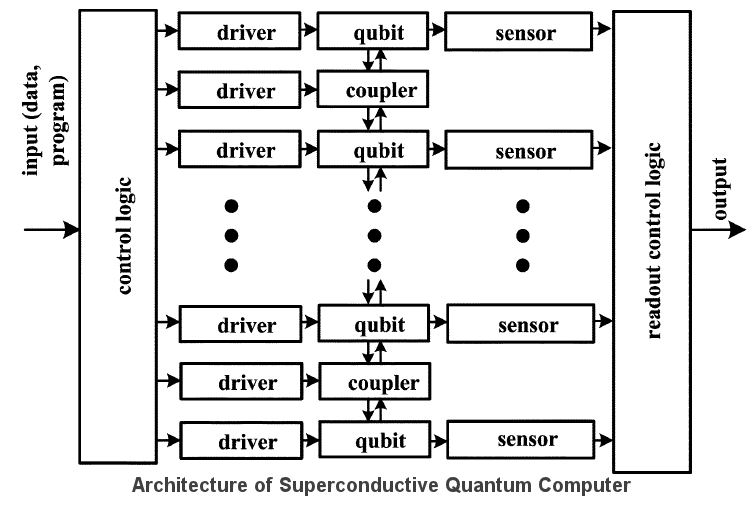
\includegraphics[scale=.5]{superconductive}
\centering
\end{figure}

\maketitle 

% Place your abstract within the special {sciabstract} environment.

\newpage

\begin{sciabstract}
\section*{Abstract}
Quantum computing is a potentially revolutionary principle which will be continued to be researched and studied for the foreseeable future as the importance of efficiency and the limit of binary computing is approached. This paper aims to provide an overview of the field of quantum computing for individuals with a minor understanding of physics, computer science, and mathematics. An introduction to quantum computing will leave the reader with a comfortable overview of the field and insight into which topic in particular they find most interesting.\par
This paper will talk briefly about the recent history of quantum computing as well as a small subset of quantum mechanicss as it relates to quantum computations and the cornerstones which currently make quantum computing possible. It aims to establish the differences between conventional and quantum computing with a goal to speak about how certain algorithms will run more efficiently and what applications in the field this can be used for. Near the end, we will look at the current issues within the field and its future importance.

\end{sciabstract}

\newpage

\tableofcontents

\newpage


% In setting up this template for *Science* papers, we've used both
% the \section* command and the \paragraph* command for topical
% divisions.  Which you use will of course depend on the type of paper
% you're writing.  Review Articles tend to have displayed headings, for
% which \section* is more appropriate; Research Articles, when they have
% formal topical divisions at all, tend to signal them with bold text
% that runs into the paragraph, for which \paragraph* is the right
% choice.  Either way, use the asterisk (*) modifier, as shown, to
% suppress numbering.

\section{History}

Quantum computing is a relatively new field in relation to computer science as a discipline with the informal start originating in the late 1970's and early 1980's as Richard Feynman speculated that quantum mechanics could not be effectively modeled through a classical computer. In accordance with Moore's law, the size of a silicon ship would continue to shrink until the individual elements were no larger than several atoms and would be subject to quantum effects at that scale. Feynman published an abstract model in 1982 in which he analyzed the outcome of using a quantum simulator in order to avoid the exponential slowdown which is common with classical computers.\cite{web}\par
In 1985, David Deutsch published a paper proving that any physical process could be, in theory, effectively rendered on a quantum computer. As a result, a quantum computer, which is able to operate in an exponential time, could provide a wide array of values for heavy data crunching, modelling of complex systems, or in the general solving NP-Complete classical problems in polynomial time.
\footnote{In computational complexity theory, a decision problem is NP-complete when it is both in NP and NP-hard. The set of NP-complete problems is often denoted by NP-C or NPC. The abbreviation NP refers to ``nondeterministic polynomial time''.\\Although any given solution to an NP-complete problem can be verified quickly (in polynomial time), there is no known efficient way to locate a solution in the first place.}
Deutsch proved a basic algorithm which will be worked through later in the paper. \par
Until 1994, the quantum computing field remained relatively unchanged until Shor was able to prove and set a method for a common NP-Hard factorization problem which could call on the benefits allowed through quantum computers, which would run in a time much shorter than what will be ever possible on classical computers.\cite{web} As a field, this momentus finding was able to push the field of research for quantum computing out of the view of the select who were performing research on the project to the public eye. Shor's algorithm will be explored later in the paper as well.\par

\section{Quantum Mechanics}

As a quick note, the material that will only be covered consists of a very small section of quantum mechanics encompassing finite dimenstional quantum mechanic where the vector spaces which represent the states of the dimension are finite in size.\par

\subsection{Double Slit Experiment}
Young's double slit experiment is one of the most foundational experiments related to the field of quantum mechanics and demonstrates the wave-particle duality of photons when conducted. Before approaching the quantum model, it is interesting to explore a classical model and the probabilities associated with it before moving on.\par
Pretend for a moment, that there is an experiment where there is a sharpshooter who is guaranteed to always shoot through one or the other open windows, with equal probability. Once the bullet passes through the window, it has an equal probability of hitting three targets. There is one target which is shared between both open windows. The probability matrix associated with this scene is shown. 
\begin{wrapfigure}{l}{0.5\textwidth}
    \centering
    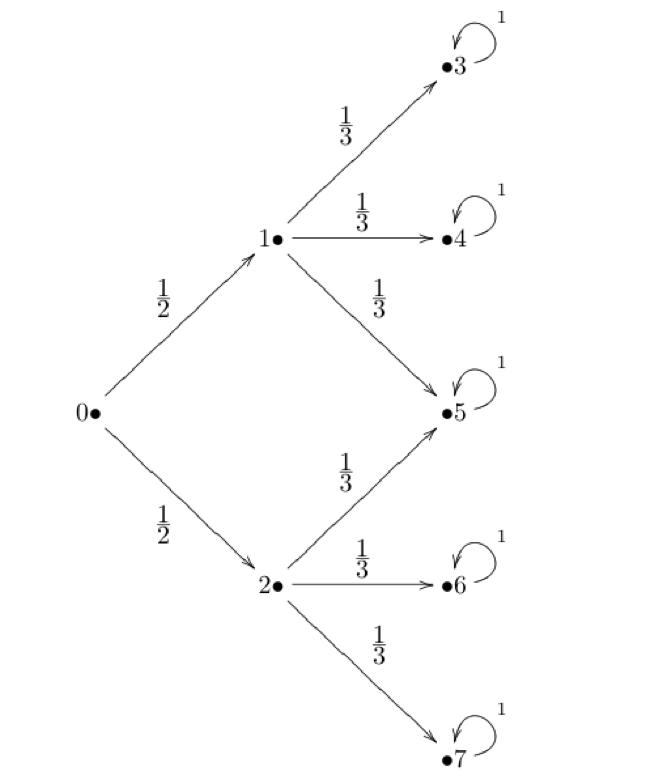
\includegraphics[width=0.5\textwidth]{classicslit}
\end{wrapfigure}
\begin{wrapfigure}{r}{0.5\textwidth}
    \centering
    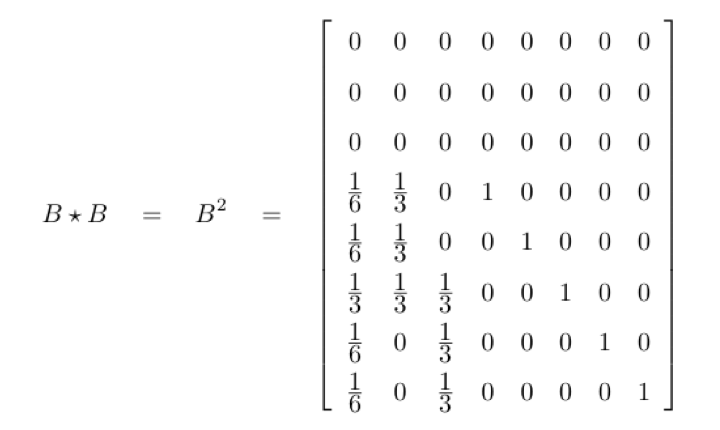
\includegraphics[width=0.5\textwidth]{classicB2}
\end{wrapfigure}
\par
By representing the data points as a matrix, it is possible to identify the probability where the bullet might be found on the next time click by simply using matrix multiplication.\cite{intro}. The matrix shown above, \textit{B}, represents the state of the system after one time click. By multiplying the matrix by itself you are able to represent the state after two time clicks. REFERENCE FIGURE 3.\par
The takeaway from this example is to show that after two time clicks the bullets will be in the state \[B^2X = [0,0,0,\frac{1}{6},\frac{1}{6},\frac{1}{3},\frac{1}{6},\frac{1}{6}]^T\]
Which means that \(B^2[5,0]\) is equivalent to \(\frac{1}{3}\). Which is the two states \(\frac{1}{6}+\frac{1}{6}\).\par

Pretend for a moment that the shooter has now been changed to a floodlight which can spread light into both of the windows with a similar setting.

\section{Qubit}
\subsection{Notation}
\subsection{Implementation}

\section{Applications}
\subsection{Implementation}
\section{Algorithms}
\subsection{Shor's Algorithm}
\subsection{Grover's Algorithm}
\subsection{Deutsch Algorithm}
\section{Error Correction and Measurement}
\section{Future of Quantum Computing}



\begin{quote}
\begin{verbatim}
However, this record of the solar nebula may have been
partly erased by the complex history of the meteorite
parent bodies, which includes collision-induced shock,
thermal metamorphism, and aqueous alteration
({\it 1, 2, 5--7\/}).
\end{verbatim}
\end{quote}


\noindent Compiled, the last two lines of the code above, of course, would give notecalls in {\it Science\/} style:

\begin{quote}
\ldots thermal metamorphism, and aqueous alteration ({\it 1, 2, 5--7\/}).
\end{quote}

Under the same luck, the author could set up his or her reference list as a simple enumeration,

\begin{quote}
\begin{verbatim}
{\bf References and Notes}

\begin{enumerate}
\item G. Gamow, {\it The Constitution of Atomic Nuclei
and Radioactivity\/} (Oxford Univ. Press, New York, 1931).
\item W. Heisenberg and W. Pauli, {\it Zeitschr.\ f.\ 
Physik\/} {\bf 56}, 1 (1929).
\end{enumerate}
\end{verbatim}
\end{quote}

\noindent yielding

\begin{quote}
{\bf References and Notes}

\begin{enumerate}
\item G. Gamow, {\it The Constitution of Atomic Nuclei and
Radioactivity\/} (Oxford Univ. Press, New York, 1931).
\item W. Heisenberg and W. Pauli, {\it Zeitschr.\ f.\ Physik} {\bf 56},
1 (1929).
\end{enumerate}
\end{quote}

That's not a solution that's likely to appeal to everyone, however ---
especially not to users of B{\small{IB}}\TeX\ \cite{inclme}.  If you
are a B{\small{IB}}\TeX\ user, we suggest that you use the
\texttt{Science.bst} bibliography style file and the
\texttt{scicite.sty} package, both of which we are downloadable from our author help site
(http://www.sciencemag.org/about/authors/prep/TeX\_help/).  You can also
generate your reference lists by using the list environment
\texttt{\{thebibliography\}} at the end of your source document; here
again, you may find the \texttt{scicite.sty} file useful.

Whether you use B{\small{IB}}\TeX\ or \texttt{\{thebibliography\}}, be
very careful about how you set up your in-text reference calls and
notecalls.  In particular, observe the following requirements:

\begin{enumerate}
\item Please follow the style for references outlined at our author
help site and embodied in recent issues of {\it Science}.  Each
citation number should refer to a single reference; please do not
concatenate several references under a single number.
\item Please cite your references and notes in text {\it only\/} using
the standard \LaTeX\ \verb+\cite+ command, not another command
driven by outside macros.
\item Please separate multiple citations within a single \verb+\cite+
command using commas only; there should be {\it no space\/}
between reference keynames.  That is, if you are citing two
papers whose bibliography keys are \texttt{keyname1} and
\texttt{keyname2}, the in-text cite should read
\verb+\cite{keyname1,keyname2}+, {\it not\/}
\verb+\cite{keyname1, keyname2}+.
\end{enumerate}

\noindent Failure to follow these guidelines could lead
to the omission of the references in an accepted paper when the source
file is translated to Word via HTML.

\section*{Handling Math, Tables, and Figures}

Following are a few things to keep in mind in coding equations,
tables, and figures for submission to {\it Science}.

\paragraph*{In-line math.}  The utility that we use for converting
from \LaTeX\ to HTML handles in-line math relatively well.  It is best
to avoid using built-up fractions in in-line equations, and going for
the more boring ``slash'' presentation whenever possible --- that is,
for \verb+$a/b$+ (which comes out as $a/b$) rather than
\verb+$\frac{a}{b}$+ (which compiles as $\frac{a}{b}$).  Likewise,
HTML isn't tooled to handle certain overaccented special characters
in-line; for $\hat{\alpha}$ (coded \verb+$\hat{\alpha}$+), for
example, the HTML translation code will return [\^{}$(\alpha)$].
Don't drive yourself crazy --- but if it's possible to avoid such
constructs, please do so.  Please do not code arrays or matrices as
in-line math; display them instead.  And please keep your coding as
\TeX-y as possible --- avoid using specialized math macro packages
like \texttt{amstex.sty}.

\paragraph*{Displayed math.} Our HTML converter sets up \TeX\
displayed equations using nested HTML tables.  That works well for an
HTML presentation, but Word chokes when it comes across a nested
table in an HTML file.  We surmount that problem by simply cutting the
displayed equations out of the HTML before it's imported into Word,
and then replacing them in the Word document using either images or
equations generated by a Word equation editor.  Strictly speaking,
this procedure doesn't bear on how you should prepare your manuscript
--- although, for reasons best consigned to a note \cite{nattex}, we'd
prefer that you use native \TeX\ commands within displayed-math
environments, rather than \LaTeX\ sub-environments.

\paragraph*{Tables.}  The HTML converter that we use seems to handle
reasonably well simple tables generated using the \LaTeX\
\texttt{\{tabular\}} environment.  For very complicated tables, you
may want to consider generating them in a word processing program and
including them as a separate file.

\paragraph*{Figures.}  Figure callouts within the text should not be
in the form of \LaTeX\ references, but should simply be typed in ---
that is, \verb+(Fig. 1)+ rather than \verb+\ref{fig1}+.  For the
figures themselves, treatment can differ depending on whether the
manuscript is an initial submission or a final revision for acceptance
and publication.  For an initial submission and review copy, you can
use the \LaTeX\ \verb+{figure}+ environment and the
\verb+\includegraphics+ command to include your PostScript figures at
the end of the compiled PostScript file.  For the final revision,
however, the \verb+{figure}+ environment should {\it not\/} be used;
instead, the figure captions themselves should be typed in as regular
text at the end of the source file (an example is included here), and
the figures should be uploaded separately according to the Art
Department's instructions.


\section*{What to Send In}

What you should send to {\it Science\/} will depend on the stage your manuscript is in:

\begin{itemize}
\item {\bf Important:} If you're sending in the initial submission of
your manuscript (that is, the copy for evaluation and peer review),
please send in {\it only\/} a PostScript or PDF version of the
compiled file (including figures).  Please do not send in the \TeX\ 
source, \texttt{.sty}, \texttt{.bbl}, or other associated files with
your initial submission.  (For more information, please see the
instructions at our Web submission site,
http://www.submit2science.org/ .)
\item When the time comes for you to send in your revised final
manuscript (i.e., after peer review), we require that you include
all source files and generated files in your upload.  Thus, if the
name of your main source document is \texttt{ltxfile.tex}, you
need to include:
\begin{itemize}
\item \texttt{ltxfile.tex}.
\item \texttt{ltxfile.aux}, the auxilliary file generated by the
compilation.
\item A PostScript file (compiled using \texttt{dvips} or some other
driver) of the \texttt{.dvi} file generated from
\texttt{ltxfile.tex}, or a PDF file distilled from that
PostScript.  You do not need to include the actual \texttt{.dvi}
file in your upload.
\item From B{\small{IB}}\TeX\ users, your bibliography (\texttt{.bib})
file, {\it and\/} the generated file \texttt{ltxfile.bbl} created
when you run B{\small{IB}}\TeX.
\item Any additional \texttt{.sty} and \texttt{.bst} files called by
the source code (though, for reasons noted earlier, we {\it
strongly\/} discourage the use of such files beyond those
mentioned in this document).
\end{itemize}
\end{itemize}

\begin{figure}
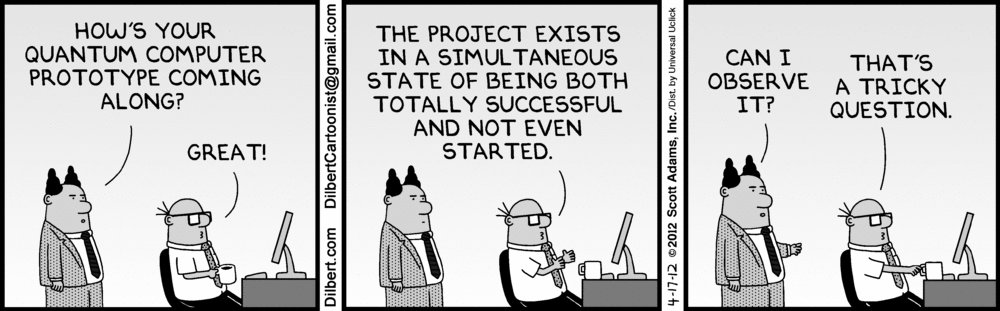
\includegraphics[scale=.5]{dilbert}
\centering
\end{figure}

% Your references go at the end of the main text, and before the
% figures.  For this document we've used BibTeX, the .bib file
% scibib.bib, and the .bst file Science.bst.  The package scicite.sty
% was included to format the reference numbers according to *Science*
% style.


\bibliography{scibib}

\bibliographystyle{Science}



% Following is a new environment, {scilastnote}, that's defined in the
% preamble and that allows authors to add a reference at the end of the
% list that's not signaled in the text; such references are used in
% *Science* for acknowledgments of funding, help, etc.

\begin{scilastnote}
\item We've included in the template file \texttt{scifile.tex} a new
environment, \texttt{\{scilastnote\}}, that generates a numbered final
citation without a corresponding signal in the text.  This environment
can be used to generate a final numbered reference containing
acknowledgments, sources of funding, and the like, per {\it Science\/}
style.
\end{scilastnote}

\newpage

\begin{thebibliography}{1}
\bibitem{pro} 
Preskill, John. ``Quantum Computing: Pro and Con.'' Diss. California Instute of Technology, 1996. Print. Covers the applications in which it will be used as well as the technical difficulties that are encountered with creating a quantum computer. Also encompasses the future of quantum computing
\bibitem{non}
Rieffel, Eleanor, and Wolfgang Polak. ``An Introduction to Quantum Computing for Non-Physicists.'' Diss. FX Palo Alto Laboratory, 2000. Print. Covers some algorithm efficiencies for conventional vs quantum computing and also covers basic applications of quantum computing in the field including cryptography.
\bibitem{web}
West, Jacob. ``The Quantum Computer.'' An Introduction to Quantum Computing. Rice University, 28 Apr. 2000. Web. 25 Oct. 2015. Provides a general purpose overview of the field of quantum computing. Includes a brief history of the field as well as current obstacles and research being done in the field.
\bibitem{intro}
Yanofsky, Noson S. ``An Introduction to Quantum Computing.'' Diss. Department of Computer and Information Science, Brooklyn College, CUNY, 2007. Print. Presents an introduction to the mathematics behind quantum computing as well as an overview of the architecture necessary for quantum computing. This paper also presents Deutsch's Algorithm which will be spoken about and overviewed.
\end{thebibliography}

\clearpage

\noindent {\bf Fig. 1.} Please do not use figure environments to set
up your figures in the final (post-peer-review) draft, do not include graphics in your
source code, and do not cite figures in the text using \LaTeX\
\verb+\ref+ commands.  Instead, simply refer to the figure numbers in
the text per {\it Science\/} style, and include the list of captions at
the end of the document, coded as ordinary paragraphs as shown in the
\texttt{scifile.tex} template file.  Your actual figure files should
be submitted separately.

\end{document}




















